%!TEX program = pdflatex
\documentclass[a4paper, 11pt]{article}

% ==================== PACKAGES ====================
\usepackage[utf8]{inputenc}
\usepackage[T1]{fontenc}
\usepackage[english]{babel}
\usepackage{amsmath, amssymb, amsfonts}
\usepackage{graphicx}
\usepackage{float}
\usepackage{booktabs}
\usepackage{array}
\usepackage{tabularx}
\usepackage{multirow}
\usepackage{geometry}
\usepackage{hyperref}
\usepackage{xcolor}
\usepackage{enumitem}
\usepackage{siunitx}
\usepackage{caption}
\usepackage{subcaption}
\usepackage{fancyhdr}
\usepackage{tcolorbox}
\usepackage{chemformula}

% ==================== GEOMETRY ====================
\geometry{
    left=2.5cm,
    right=2.5cm,
    top=2.5cm,
    bottom=2.5cm,
    headheight=14pt
}

% ==================== COLORS ====================
\definecolor{darkblue}{RGB}{0, 51, 102}
\definecolor{lightblue}{RGB}{230, 240, 250}
\definecolor{darkgreen}{RGB}{0, 100, 0}

% ==================== HYPERREF SETUP ====================
\hypersetup{
    colorlinks=true,
    linkcolor=darkblue,
    urlcolor=darkblue,
    citecolor=darkblue
}

% ==================== HEADER/FOOTER ====================
\pagestyle{fancy}
\fancyhf{}
\fancyhead[L]{\textit{Fiber Optics - Production of Optical Fibers}}
\fancyhead[R]{\textit{FO9 Summary}}
\fancyfoot[C]{\thepage}
\renewcommand{\headrulewidth}{0.4pt}

% ==================== CUSTOM BOXES ====================
\newtcolorbox{keypoint}{
    colback=lightblue,
    colframe=darkblue,
    fonttitle=\bfseries,
    title=Key Point
}

\newtcolorbox{formula}{
    colback=yellow!10,
    colframe=orange!80!black,
    fonttitle=\bfseries,
    title=Formula
}

% ==================== DOCUMENT ====================
\begin{document}

% ==================== TITLE PAGE ====================
\begin{titlepage}
    \centering
    \vspace*{2cm}
    
    {\Huge\bfseries Production of Optical Fibers\par}
    \vspace{0.5cm}
    {\Large\textit{From Preform to Cable}\par}
    
    \vspace{2cm}
    
    {\large Summary of Lecture Notes by Luca Palmieri\par}
    {\large Course: Fiber Optics\par}
    {\large Academic Year 2019/2020\par}
    
    \vspace{3cm}
    
    \begin{abstract}
    This document provides a comprehensive technical summary of the optical fiber production process, covering the fundamental structure of optical fibers (core/cladding), propagation principles, and the three main production phases: preform manufacturing, fiber drawing, and cabling. Special emphasis is placed on Chemical Vapor Deposition (CVD) techniques including MCVD, PCVD, OVD, and VAD, with detailed analysis of their chemical reactions, advantages, and disadvantages.
    \end{abstract}
    
    \vfill
    
    {\large ICT Engineering - Summary Document\par}
    {\large January 2026\par}
\end{titlepage}

\tableofcontents
\newpage

% ==================== INTRODUCTION ====================
\section{Introduction to Optical Fiber Structure}

\subsection{Core and Cladding Structure}

Optical fibers are cylindrical waveguides composed of two main concentric regions:

\begin{itemize}[leftmargin=*]
    \item \textbf{Core (Nucleo):} The central region where light propagates. It has a slightly higher refractive index than the cladding.
    \item \textbf{Cladding (Mantello):} The outer layer surrounding the core, with a lower refractive index.
\end{itemize}

\begin{keypoint}
The refractive index difference between core and cladding enables light confinement through total internal reflection.
\end{keypoint}

The typical parameters for telecommunication fibers are:

\begin{table}[H]
    \centering
    \caption{Typical optical fiber parameters}
    \label{tab:fiber_params}
    \begin{tabular}{lcc}
        \toprule
        \textbf{Parameter} & \textbf{Core} & \textbf{Cladding} \\
        \midrule
        Refractive index $n$ & $n_{co} \approx 1.466$ & $n_{cl} \approx 1.444$ \\
        Diameter $d$ & $d_{co} \approx 6 \div 65~\si{\micro\meter}$ & $d_{cl} \approx 125~\si{\micro\meter}$ \\
        \bottomrule
    \end{tabular}
\end{table}

\begin{figure}[H]
    \centering
    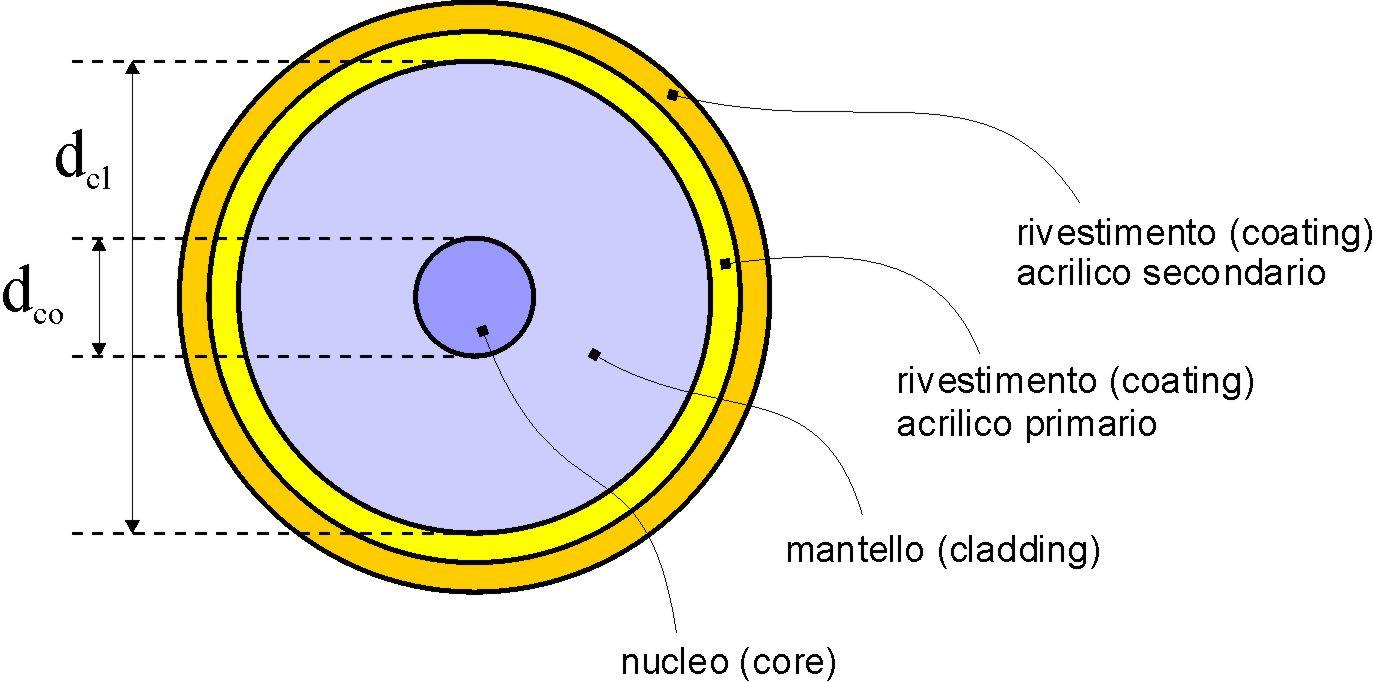
\includegraphics[width=0.7\textwidth]{Images/fig-001.png}
    \caption{Cross-sectional view of an optical fiber showing the core ($d_{co}$), cladding ($d_{cl}$), and the primary and secondary acrylic coatings. The core has a higher refractive index than the cladding, enabling light confinement.}
    \label{fig:fiber_cross_section}
\end{figure}

\subsection{Propagation Principles}

During propagation, light is mainly confined in the core. The confinement mechanism can be explained at two levels of approximation:

\begin{enumerate}[leftmargin=*]
    \item \textbf{First-order approximation:} Total internal reflection (TIR) at the core-cladding interface.
    \item \textbf{More accurate description:} Modal analysis, where light propagates as discrete modes.
\end{enumerate}

\begin{figure}[H]
    \centering
    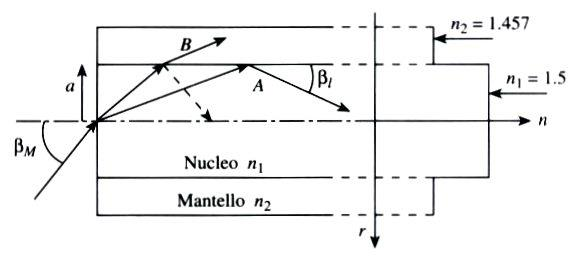
\includegraphics[width=0.65\textwidth]{Images/fig-000.png}
    \caption{Ray propagation in an optical fiber showing total internal reflection. The ray enters the fiber at an angle and is reflected at the core-cladding interface. The critical angle $\beta_M$ determines the maximum acceptance angle.}
    \label{fig:ray_propagation}
\end{figure}

The modes of propagation include:
\begin{itemize}
    \item $\text{TE}_{0,p}$ and $\text{TM}_{0,p}$ modes (transverse electric and magnetic)
    \item $\text{HE}_{m,p}$ and $\text{EH}_{m,p}$ hybrid modes
\end{itemize}

\subsection{Refractive Index Profile}

The propagation properties of an optical fiber are defined by its \textbf{refractive index profile}. Different profiles yield different fiber types with specific characteristics:

\begin{figure}[H]
    \centering
    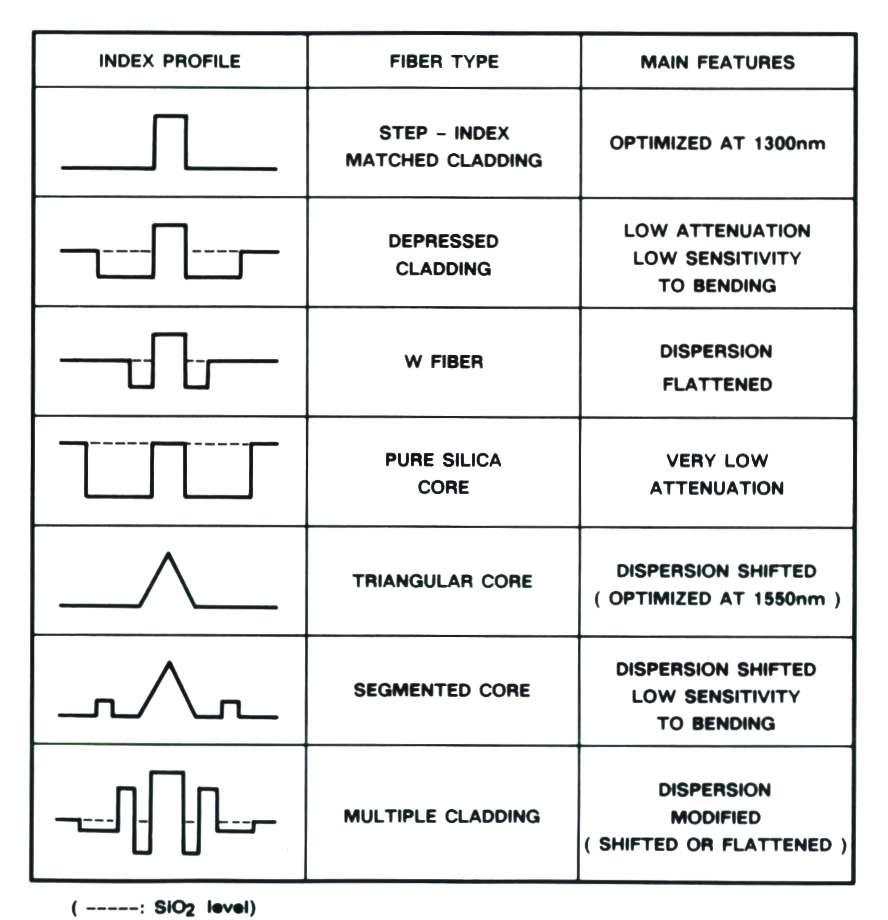
\includegraphics[width=0.85\textwidth]{Images/fig-002.png}
    \caption{Various refractive index profiles and their corresponding fiber types. Each profile optimizes different transmission properties such as dispersion, attenuation, and bending sensitivity. The dashed line indicates the pure silica ($\ch{SiO2}$) refractive index level.}
    \label{fig:index_profiles}
\end{figure}

\subsection{Fiber Materials}

Optical fibers can be manufactured from two main material categories:

\begin{enumerate}[leftmargin=*]
    \item \textbf{Silica ($\ch{SiO2}$) fibers:} Used in all high-capacity telecommunication systems due to their superior optical properties (low attenuation, low dispersion).
    
    \item \textbf{Polymer Optical Fibers (POF):} Higher attenuation but cheaper to produce and install. Limited to small networks such as buildings, cars, and airplanes.
\end{enumerate}

\begin{figure}[H]
    \centering
    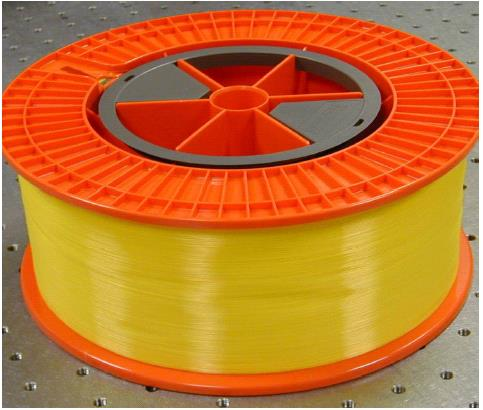
\includegraphics[width=0.5\textwidth]{Images/fig-003.png}
    \caption{Spool of polymer optical fiber (POF). POF is recognizable by its characteristic yellow/orange color and larger core diameter compared to silica fibers.}
    \label{fig:pof_spool}
\end{figure}

% ==================== PRODUCTION PHASES ====================
\section{Production Phases Overview}

The production of an optical fiber cable consists of \textbf{three main phases}:

\begin{enumerate}[leftmargin=*, label=\textbf{\arabic*.}]
    \item \textbf{Preform Production:} Manufacturing of a silica cylinder that reproduces, in a larger scale, the targeted refractive index profile.
    
    \item \textbf{Fiber Drawing:} Heating the preform to its viscous state and drawing it into a thin fiber.
    
    \item \textbf{Cabling:} Application of protective layers to the fiber for mechanical protection during installation and operation.
\end{enumerate}

\begin{table}[H]
    \centering
    \caption{Summary of production phases}
    \label{tab:production_phases}
    \begin{tabularx}{\textwidth}{lXX}
        \toprule
        \textbf{Phase} & \textbf{Description} & \textbf{Key Parameters} \\
        \midrule
        Preform & Silica cylinder with scaled refractive index profile & Length: $\sim 1~\si{m}$, Diameter: few to tens of cm \\
        Drawing & Heating and pulling the preform into fiber & Speed: up to several tens of m/s \\
        Cabling & Application of protective sheathings & Final diameter: $0.250~\si{mm}$ (bare fiber) \\
        \bottomrule
    \end{tabularx}
\end{table}

% ==================== PREFORM PRODUCTION ====================
\section{Phase 1: Preform Production}

\subsection{Overview}

The preform is a silica cylinder that reproduces in a larger scale the targeted refractive index profile. Typical preform characteristics:

\begin{itemize}
    \item Length: approximately 1 meter
    \item Diameter: from a few up to several tens of centimeters
    \item Yield: a single preform can produce up to \textbf{several hundreds of kilometers} of optical fiber
\end{itemize}

\subsection{Production Techniques}

There are two main techniques to produce the preform:

\subsubsection{Chemical Vapor Deposition (CVD)}

This is the most common technique, enabling the production of silica with extremely high purity and tight control over dopant concentration. CVD processes include MCVD, PCVD, OVD, and VAD.

\subsubsection{Sol-Gel Process}

In this technique, silica and other constituents are first held together by a gel matrix and then sintered into the final preform. While it offers higher yield compared to CVD, the final quality is lower. Sol-gel is sometimes used for the outer cladding layers.

% ==================== CVD ====================
\section{Chemical Vapor Deposition (CVD) Techniques}

\subsection{Fundamental Chemistry}

CVD is a technique used to produce materials of the utmost purity, widely employed in the semiconductor industry. For silica optical fibers, CVD is based on the \textbf{oxidation of silicon tetrachloride}:

\begin{formula}
\textbf{Silica formation reaction (irreversible):}
\begin{equation}
    \ch{SiCl4 + O2 -> SiO2 + 2Cl2}
    \label{eq:silica_cvd}
\end{equation}
\end{formula}

\begin{itemize}
    \item \textbf{Reactants:} Silicon tetrachloride ($\ch{SiCl4}$) vapors, oxygen ($\ch{O2}$)
    \item \textbf{Temperature:} 1200--1600°C
    \item \textbf{Products:} Silica soot ($\ch{SiO2}$) and molecular chlorine ($\ch{Cl2}$)
    \item \textbf{Reaction type:} Irreversible
\end{itemize}

\begin{keypoint}
The silica produced via CVD is \textbf{more pure than the original reactants}. This is possible because silicon tetrachloride evaporates at much lower temperatures compared to typical contaminants.
\end{keypoint}

The refractive index of pure silica at 1550 nm is $n = 1.444$.

\subsection{Dopants and Refractive Index Control}

The refractive index profile is defined by \textbf{doping silica} in a controlled manner. Different dopants can either increase or decrease the refractive index:

\begin{figure}[H]
    \centering
    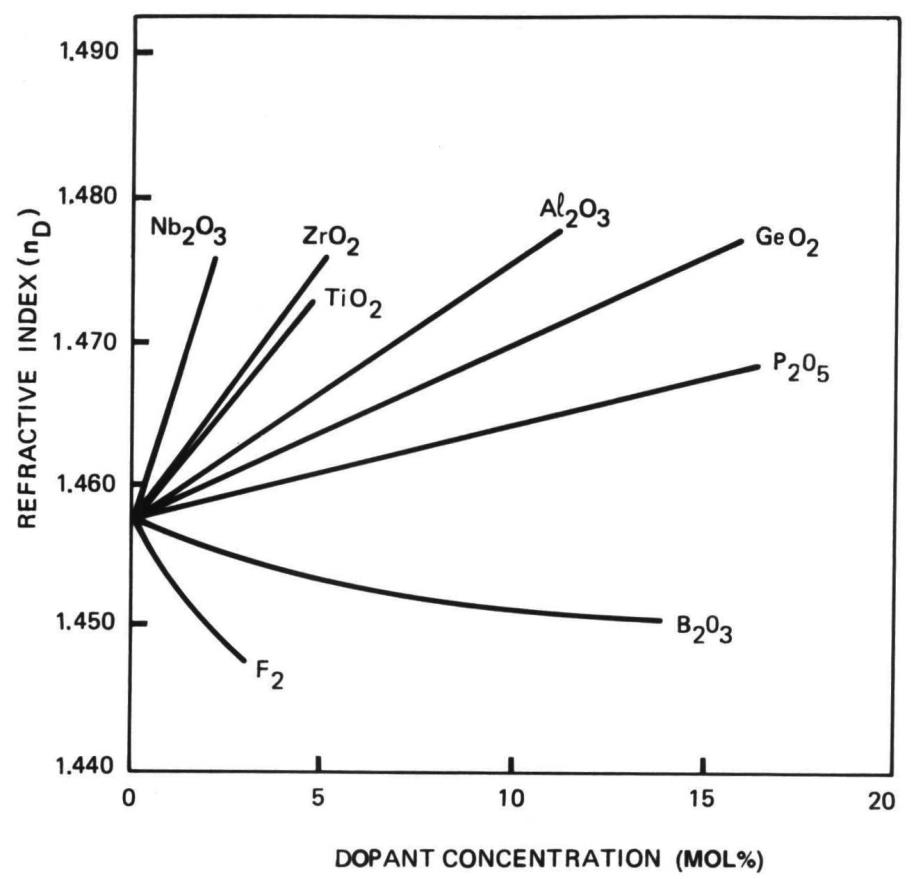
\includegraphics[width=0.7\textwidth]{Images/fig-004.png}
    \caption{Effect of different dopants on the refractive index of silica as a function of dopant concentration (mol\%). Germanium dioxide ($\ch{GeO2}$) and other compounds increase the refractive index, while fluorine ($\ch{F2}$) and boron trioxide ($\ch{B2O3}$) decrease it.}
    \label{fig:dopants_effect}
\end{figure}

The most common dopant is \textbf{germanium dioxide ($\ch{GeO2}$)}, obtained through a similar oxidation reaction:

\begin{formula}
\textbf{Germanium dioxide formation (reversible):}
\begin{equation}
    \ch{GeCl4 + O2 <=> GeO2 + 2Cl2}
    \label{eq:geo2_cvd}
\end{equation}
\end{formula}

\begin{keypoint}
Unlike the silica reaction, the $\ch{GeO2}$ formation is \textbf{reversible}. The chlorine ($\ch{Cl2}$) produced from $\ch{SiCl4}$ oxidation shifts the equilibrium to the left, hindering $\ch{GeCl4}$ oxidation. This poses technical challenges in achieving high germanium concentrations.
\end{keypoint}

\subsection{Classification of CVD Techniques}

CVD techniques are divided into two main classes:

\begin{table}[H]
    \centering
    \caption{Classification of CVD techniques}
    \label{tab:cvd_classification}
    \begin{tabularx}{\textwidth}{lXX}
        \toprule
        \textbf{Class} & \textbf{Description} & \textbf{Techniques} \\
        \midrule
        \textbf{IVPO} (Inside Vapor Phase Oxidation) & Reaction occurs \textbf{inside} a quartz cylinder that acts as support and is eventually incorporated into the preform & MCVD (Bell Labs, 1974), PCVD (Philips, 1976) \\
        \midrule
        \textbf{OVPO} (Outside Vapor Phase Oxidation) & Reaction occurs \textbf{outside} a supporting bar that will not be part of the final preform & OVD (Corning, 1972), VAD (NTT, 1977) \\
        \bottomrule
    \end{tabularx}
\end{table}

% ==================== MCVD ====================
\subsection{MCVD: Modified Chemical Vapor Deposition}

\textbf{MCVD} (Modified Chemical Vapor Deposition) was developed by Bell Labs/AT\&T in 1974 and is one of the most widely used techniques.

\subsubsection{Process Description}

\begin{figure}[H]
    \centering
    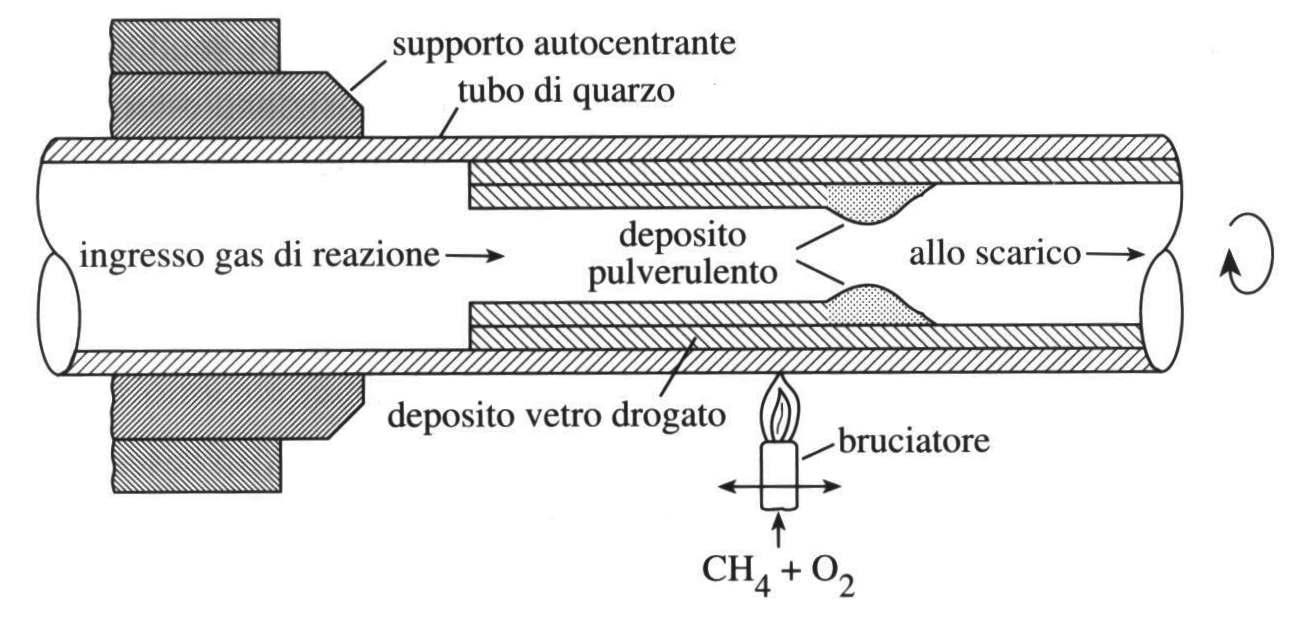
\includegraphics[width=0.85\textwidth]{Images/fig-005.png}
    \caption{Schematic of the MCVD process showing the quartz tube, gas flow, burner, and soot deposition. The reactant gases flow through the tube while a burner travels along its length, activating the oxidation reaction.}
    \label{fig:mcvd_schematic}
\end{figure}

The MCVD process consists of the following steps:

\begin{enumerate}[leftmargin=*]
    \item The reactant gases ($\ch{SiCl4}$, $\ch{GeCl4}$, $\ch{O2}$ plus other additives) move with \textbf{laminar flow} along a cylindrical quartz tube, which is kept in rotation around its axis.
    
    \item A \textbf{burner} travels along the tube at the same speed as the gases. Upon reaching the tube end, it quickly returns to the input and starts again.
    
    \item The heat delivered by the burner increases the temperature above \textbf{1200°C}, activating the oxidizing reaction and producing silica soot (or doped silica soot).
    
    \item Due to gas momentum and thermal gradient, the soot deposits on the tube's inner wall \textbf{in front of the burner}, forming a porous layer.
    
    \item As the burner proceeds, it reaches the porous layer, \textbf{heating and sintering} it. A thin layer of silica glass (thickness: 15--100 $\mu$m) is deposited at each burner passage.
    
    \item When the central bore becomes small enough, the gas flow is stopped and the burner motion is slowed down to overheat the preform and \textbf{collapse the central bore}.
\end{enumerate}

\begin{figure}[H]
    \centering
    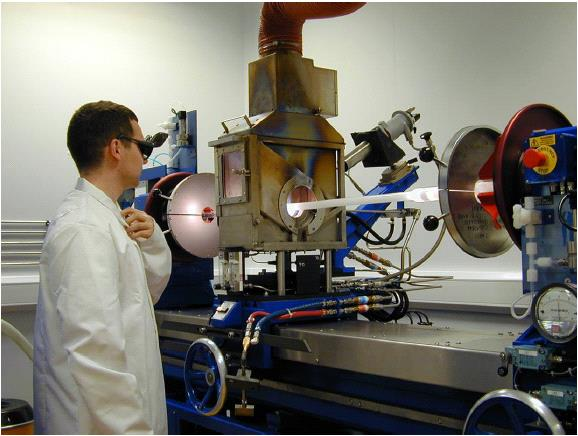
\includegraphics[width=0.7\textwidth]{Images/fig-007.png}
    \caption{Laboratory setup for MCVD process showing the rotating quartz tube, burner, and the glowing preform during deposition. The operator monitors the process to ensure uniform layer deposition.}
    \label{fig:mcvd_lab}
\end{figure}

\subsubsection{Advantages and Disadvantages}

\begin{table}[H]
    \centering
    \caption{MCVD: Advantages and Disadvantages}
    \label{tab:mcvd_pros_cons}
    \begin{tabularx}{\textwidth}{X|X}
        \toprule
        \textbf{Advantages} & \textbf{Disadvantages} \\
        \midrule
        Relatively simple and economical & Slow deposition speed (0.5--2 g/min) \\
        \addlinespace
        One of the most diffused techniques & Low efficiency: only 50\% of silica and 10--20\% of $\ch{GeO2}$ deposits \\
        \addlinespace
        & Symmetry of supporting cylinder critically impacts fiber quality \\
        \addlinespace
        & Central index dip due to $\ch{GeCl4}$ oxidation inhibition \\
        \addlinespace
        & OH$^-$ ions permanently embedded, increasing attenuation \\
        \bottomrule
    \end{tabularx}
\end{table}

% ==================== PCVD ====================
\subsection{PCVD: Plasma Chemical Vapor Deposition}

\textbf{PCVD} (Plasma Chemical Vapor Deposition) was developed by Philips in 1976. It follows the same principle as MCVD but uses a different heating mechanism.

\subsubsection{Process Description}

\begin{figure}[H]
    \centering
    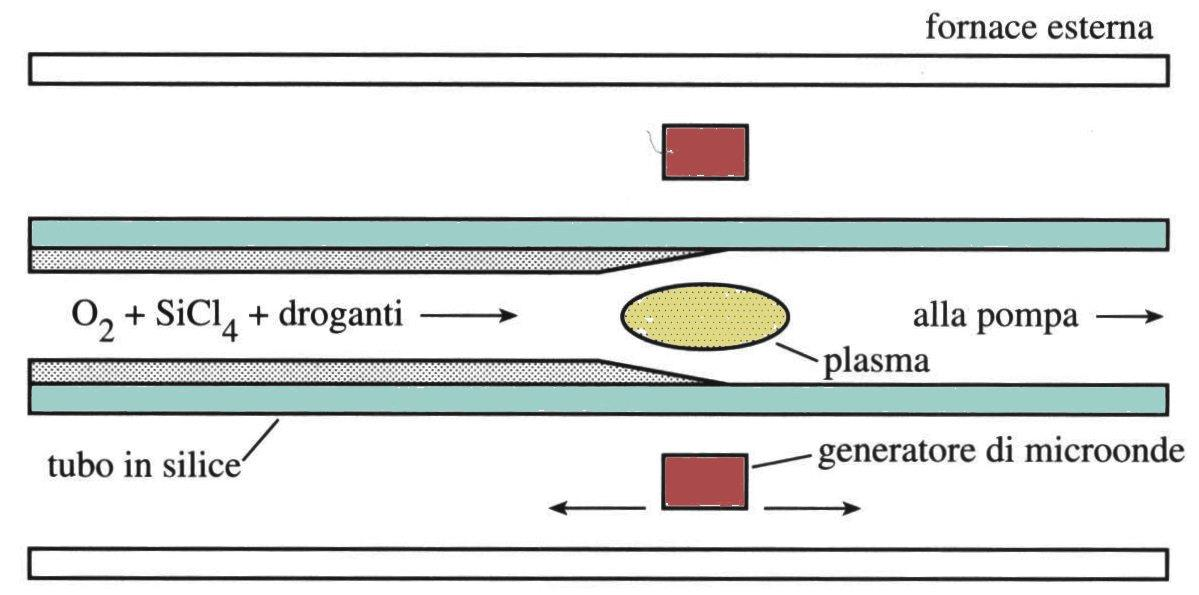
\includegraphics[width=0.8\textwidth]{Images/fig-008.png}
    \caption{Schematic of the PCVD process. A microwave generator creates a plasma inside the silica tube, causing soot formation and deposition. An external furnace maintains the tube at high temperature to prevent thermal shocks.}
    \label{fig:pcvd_schematic}
\end{figure}

The key difference from MCVD:

\begin{itemize}
    \item The burner is replaced by a \textbf{microwave generator} operating at approximately \textbf{2.45 GHz}
    \item The microwaves induce a \textbf{plasma} in the reacting gases, causing silica soot to form and precipitate
    \item An \textbf{external heater} keeps the entire tube at high temperature to avoid thermal shocks
\end{itemize}

\subsubsection{Advantages and Disadvantages}

\begin{table}[H]
    \centering
    \caption{PCVD: Advantages and Disadvantages}
    \label{tab:pcvd_pros_cons}
    \begin{tabularx}{\textwidth}{X|X}
        \toprule
        \textbf{Advantages} & \textbf{Disadvantages} \\
        \midrule
        High deposition speed (2--3 g/min) & More expensive than MCVD \\
        \addlinespace
        High efficiency: 100\% silica, 80\% $\ch{GeO2}$ deposited & Cylindrical symmetry depends on the support \\
        \addlinespace
        Extremely high resolution in index profile (layers $\sim$1 $\mu$m thick) & OH$^-$ ions permanently embedded \\
        \bottomrule
    \end{tabularx}
\end{table}

% ==================== OVD ====================
\subsection{OVD: Outside Vapor Deposition}

\textbf{OVD} (Outside Vapor Deposition) was developed by Corning in 1972 and is an OVPO technique.

\subsubsection{Process Description}

\begin{figure}[H]
    \centering
    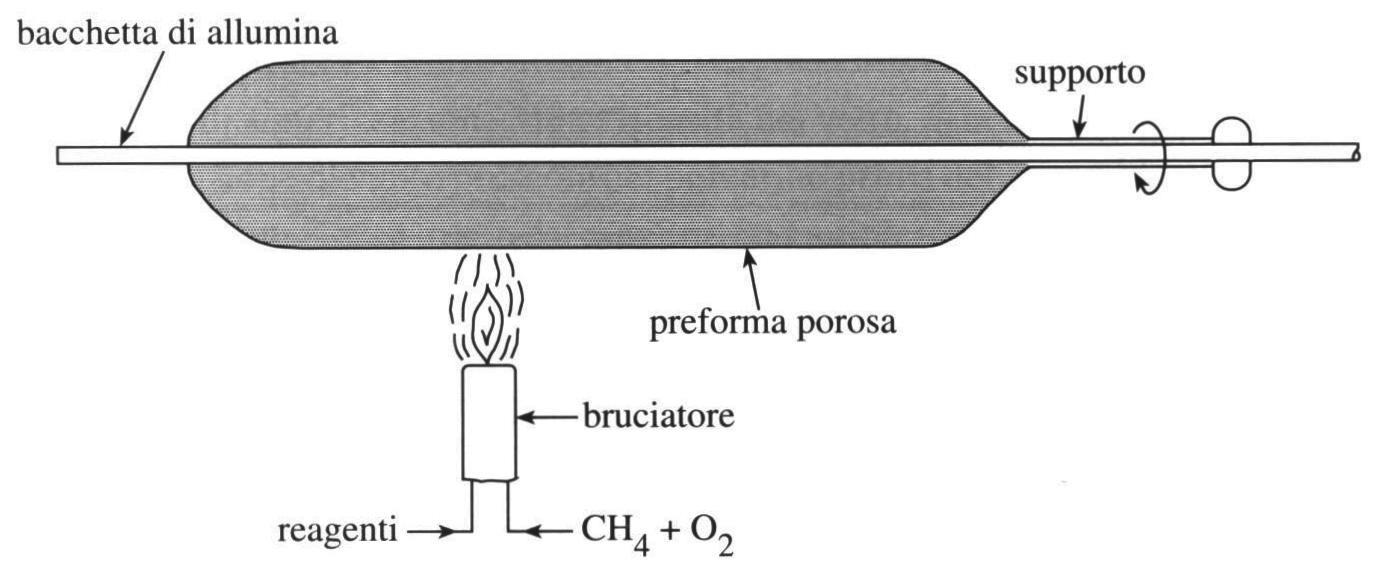
\includegraphics[width=0.7\textwidth]{Images/fig-009.png}
    \caption{Schematic of the OVD process. A thin alumina or graphite bar is rotated while exposed to a burner flame. Silica soot forms in the flame and adheres to the bar, growing a porous preform.}
    \label{fig:ovd_schematic}
\end{figure}

The OVD process consists of the following steps:

\begin{enumerate}[leftmargin=*]
    \item A thin bar of refractive material (\textbf{alumina or graphite}) is kept in rotation and moved back and forth while being exposed to a fixed burner flame.
    
    \item A mix of reactants ($\ch{SiCl4}$, $\ch{GeCl4}$, plus additives) and combustibles (\textbf{methane and oxygen}) are conveyed to the burner:
    \begin{equation}
        \ch{CH4 + O2 -> combustion}
    \end{equation}
    
    \item Silica soot (particle diameter $\approx 0.1~\mu$m) forms in the flame.
    
    \item The soot adheres to the bar, growing a \textbf{white porous preform} with density about 15--20\% of vitreous silica (2.2 g/cm³). Each layer is $\sim$100 $\mu$m thick.
    
    \item Once completed, the supporting bar is removed and the preform is inserted into furnaces at different temperatures, saturated with helium.
    
    \item \textbf{Drying phase} at $\sim$500°C: Helium gas flows through the porous structure, mechanically removing OH$^-$ ions.
    
    \item \textbf{Sintering phase} at $\sim$1500°C: The preform is sintered and the central hole is collapsed.
\end{enumerate}

\begin{figure}[H]
    \centering
    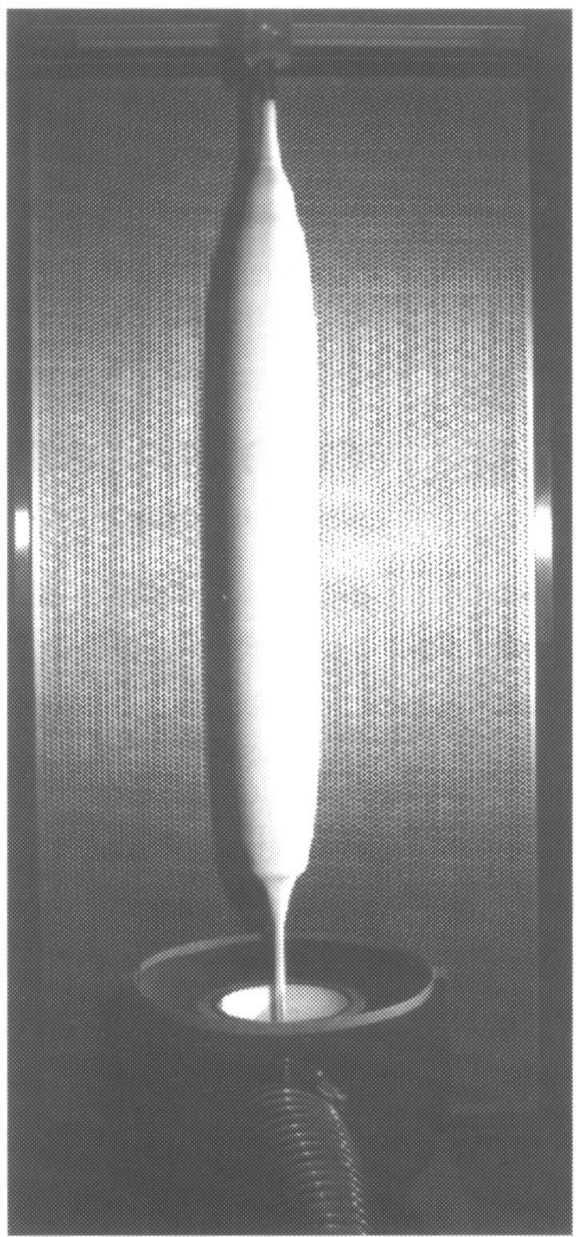
\includegraphics[width=0.45\textwidth]{Images/fig-010.png}
    \caption{OVD preform during the sintering process. The porous preform is heated to high temperature, causing it to become transparent as voids are eliminated and the material densifies.}
    \label{fig:ovd_sintering}
\end{figure}

\subsubsection{Advantages and Disadvantages}

\begin{table}[H]
    \centering
    \caption{OVD: Advantages and Disadvantages}
    \label{tab:ovd_pros_cons}
    \begin{tabularx}{\textwidth}{X|X}
        \toprule
        \textbf{Advantages} & \textbf{Disadvantages} \\
        \midrule
        High deposition speed (up to 10 g/min) & More difficult to implement and manage than MCVD \\
        \addlinespace
        High efficiency (water from $\ch{CH4}$ combustion reacts with chlorine, forming HCl and $\ch{O2}$, easing $\ch{GeCl4}$ oxidation) & Process must occur in clean rooms to avoid contamination \\
        \addlinespace
        Drying phase drastically reduces OH$^-$ contamination & \\
        \bottomrule
    \end{tabularx}
\end{table}

% ==================== VAD ====================
\subsection{VAD: Vapor Axial Deposition}

\textbf{VAD} (Vapor Axial Deposition) was developed by NTT in 1977 and is an OVPO technique optimized for continuous production.

\subsubsection{Process Description}

\begin{figure}[H]
    \centering
    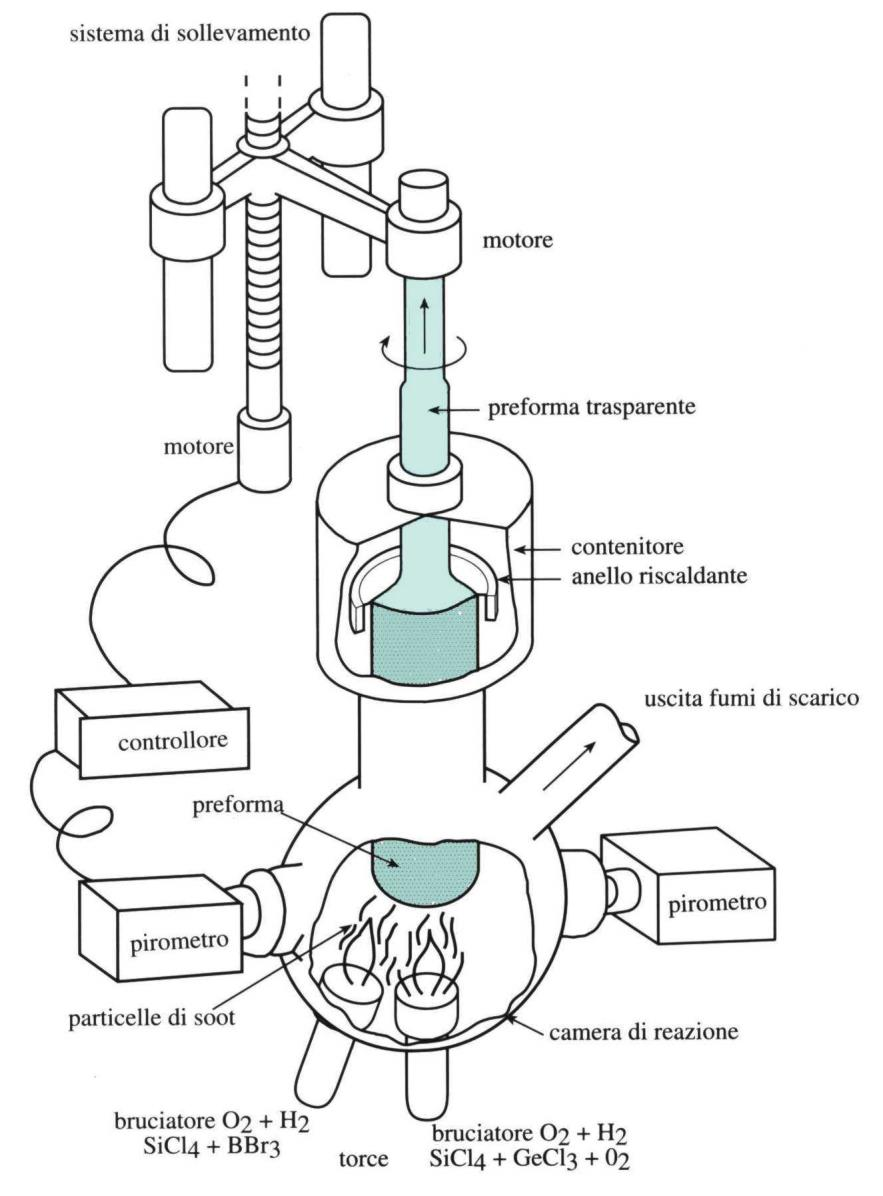
\includegraphics[width=0.65\textwidth]{Images/fig-011.png}
    \caption{Detailed schematic of the VAD process showing the lifting system, motors, heating ring, reaction chamber, burners, and pyrometers. The preform grows axially as the support moves slowly upward.}
    \label{fig:vad_schematic}
\end{figure}

The VAD process operates as follows:

\begin{enumerate}[leftmargin=*]
    \item A \textbf{silica sphere} is inserted in a reaction chamber, attached to a support that rotates and slowly moves \textbf{upward}.
    
    \item The sphere is exposed to the flames of a set of \textbf{fixed burners}.
    
    \item As in OVD, reactants and combustibles are conveyed to the burners, forming soot that adheres to the sphere and grows a \textbf{porous preform axially}.
    
    \item As the support moves upward, the preform enters other chambers where it is:
    \begin{itemize}
        \item \textbf{Dried} (to remove OH$^-$ ions)
        \item \textbf{Sintered} (to consolidate the glass)
    \end{itemize}
\end{enumerate}

\subsubsection{Advantages and Disadvantages}

\begin{table}[H]
    \centering
    \caption{VAD: Advantages and Disadvantages}
    \label{tab:vad_pros_cons}
    \begin{tabularx}{\textwidth}{X|X}
        \toprule
        \textbf{Advantages} & \textbf{Disadvantages} \\
        \midrule
        High deposition speed (up to 10 g/min) & More complex to implement than MCVD \\
        \addlinespace
        High efficiency (HCl formation eases $\ch{GeCl4}$ oxidation) & Index profile cannot be easily changed (set by burner position and flame fluidodynamics) \\
        \addlinespace
        Drying phase removes almost all OH$^-$ ions & \\
        \addlinespace
        Production occurs in sealed, controlled environment & \\
        \addlinespace
        Allows production of large preforms (up to 400 km of fiber each) & \\
        \bottomrule
    \end{tabularx}
\end{table}

% ==================== CVD COMPARISON ====================
\subsection{Comparison of CVD Techniques}

\begin{table}[H]
    \centering
    \caption{Comparative summary of CVD techniques}
    \label{tab:cvd_comparison}
    \begin{tabularx}{\textwidth}{lcccc}
        \toprule
        \textbf{Parameter} & \textbf{MCVD} & \textbf{PCVD} & \textbf{OVD} & \textbf{VAD} \\
        \midrule
        Type & IVPO & IVPO & OVPO & OVPO \\
        Deposition rate (g/min) & 0.5--2 & 2--3 & up to 10 & up to 10 \\
        $\ch{SiO2}$ efficiency (\%) & 50 & 100 & High & High \\
        $\ch{GeO2}$ efficiency (\%) & 10--20 & 80 & High & High \\
        OH$^-$ removal & No & No & Yes & Yes \\
        Layer thickness ($\mu$m) & 15--100 & $\sim$1 & $\sim$100 & -- \\
        Complexity & Low & Medium & Medium & High \\
        Fiber yield (km/preform) & Low & Low & Medium & Up to 400 \\
        \bottomrule
    \end{tabularx}
\end{table}

% ==================== DRAWING ====================
\section{Phase 2: Fiber Drawing}

\subsection{Drawing Tower Components}

The preform is drawn into a fiber on specifically built \textbf{drawing towers}. The main components are:

\begin{enumerate}[leftmargin=*]
    \item \textbf{Moving support} to hang the preform
    \item \textbf{Furnace} (heated to $\sim$2000°C)
    \item \textbf{Cooling tube}
    \item \textbf{Diameter monitoring} system
    \item \textbf{Coating device} to apply resins
    \item \textbf{UV lamps} to polymerize the resins
    \item \textbf{Spinner} (optional) for improved symmetry
    \item \textbf{Capstan} to control drawing speed
\end{enumerate}

Tower heights typically range from \textbf{5 to 25 meters}. Taller towers allow higher production speeds.

\subsection{Drawing Process}

The drawing process follows these stages:

\begin{enumerate}[leftmargin=*]
    \item The preform is hung on a support that slowly lowers it into the furnace, where it is heated close to the silica melting temperature ($\sim$2000°C). Modern furnaces are metal hollow cylinders heated by \textbf{magnetic induction}.
    
    \item As the preform softens, a drop of silica falls due to gravity, initiating the drawing process.
    
    \item The drop and connected fiber are guided by hand along the tower until the capstan. Afterwards, the process continues under \textbf{automatic control}.
    
    \item Out of the furnace, the fiber is cooled in cooling tubes with flows of inert gases (such as helium).
\end{enumerate}

\subsection{Diameter Control and Mass Conservation}

One of the most critical parameters is the \textbf{fiber diameter}, which influences propagation characteristics. The diameter is constantly monitored along the tower.

\begin{formula}
\textbf{Mass Conservation Equation:}

Let $D_p$ be the preform diameter, $d_f$ the fiber diameter, $V_p$ the speed at which the preform enters the furnace, and $v_f$ the drawing speed (controlled by capstan rotation). Mass conservation implies:

\begin{equation}
    D_p^2 \cdot V_p = d_f^2 \cdot v_f
    \label{eq:mass_conservation}
\end{equation}

Solving for fiber diameter:
\begin{equation}
    d_f = D_p \sqrt{\frac{V_p}{v_f}}
    \label{eq:fiber_diameter}
\end{equation}
\end{formula}

\begin{keypoint}
Fiber diameter can be controlled by adjusting the \textbf{drawing speed} ($v_f$). Increasing capstan rotation speed reduces the fiber diameter.
\end{keypoint}

The fiber diameter is measured by analyzing the \textbf{interference patterns} created when illuminating the fiber from its side.

\subsection{Coating Application}

\begin{figure}[H]
    \centering
    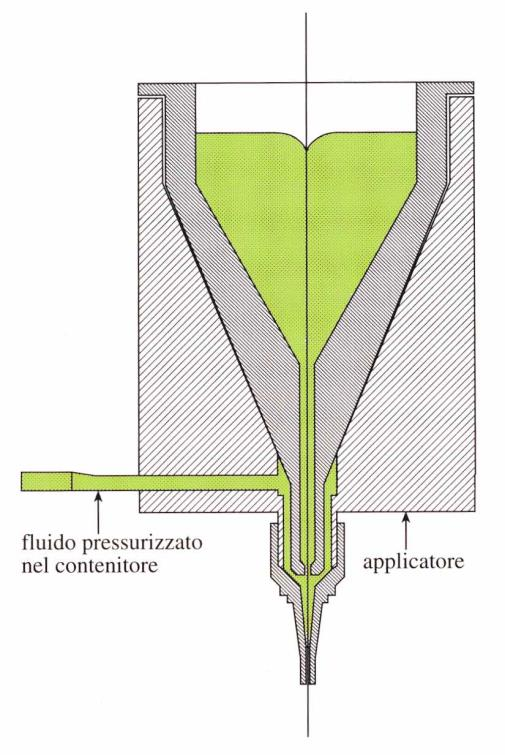
\includegraphics[width=0.4\textwidth]{Images/fig-017.png}
    \caption{Cross-sectional schematic of the coating applicator. The fiber passes through pressurized acrylic resin, which coats it uniformly. The coating is then cured by UV lamps.}
    \label{fig:coating_applicator}
\end{figure}

The cooled fiber passes through a coating device that applies \textbf{acrylic resin}. The resin is then polymerized by exposure to UV lamps. Standard telecommunication fibers have \textbf{two layers of coating}:

\begin{itemize}
    \item \textbf{First layer (inner):} Rather soft, almost jelly-like. Provides mechanical isolation from the external environment and makes the outer coating easy to remove.
    
    \item \textbf{Second layer (outer):} Provides mechanical protection with low friction coefficient to facilitate cabling and winding.
\end{itemize}

The final outer diameter is \textbf{250 $\mu$m} for standard telecom fibers.

\begin{figure}[H]
    \centering
    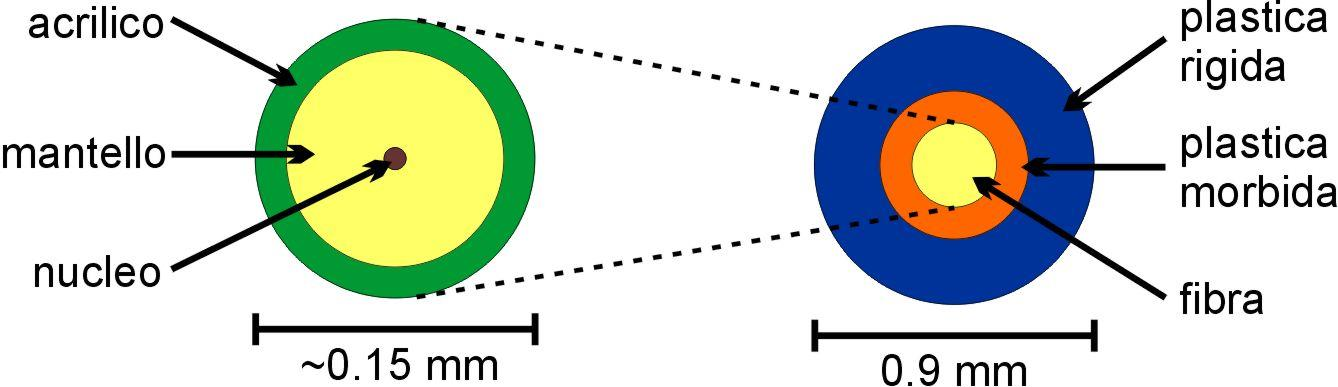
\includegraphics[width=0.6\textwidth]{Images/fig-022.png}
    \caption{Comparison of coated fiber cross-sections. Left: bare fiber with primary coating ($\sim$0.15 mm). Right: 900-micron buffered fiber with additional Teflon protection (0.9 mm diameter).}
    \label{fig:coating_comparison}
\end{figure}

\subsection{Spinner for Polarization Mode Dispersion Reduction}

For high-quality fiber production, a \textbf{spinner} is inserted before the capstan. The spinner induces a controlled rotation of the fiber around its axis, which:

\begin{itemize}
    \item Improves the \textbf{cylindrical symmetry} of the fiber
    \item Reduces \textbf{polarization mode dispersion (PMD)}
    \item Can achieve spin rates of \textbf{several hundred turns per second}
\end{itemize}

\subsection{Drawing Speed and Control}

At the bottom of the tower, the fiber is wound on the \textbf{capstan}, whose rotation speed controls the fiber diameter. The tower is managed automatically by controlling:

\begin{itemize}
    \item Furnace temperature
    \item Preform feed speed
    \item Capstan speed
\end{itemize}

Drawing speeds can be as high as \textbf{several tens of meters per second} for telecom fibers.

% ==================== CABLING ====================
\section{Phase 3: Cabling}

\subsection{Need for Protection}

Despite a silica wire being stiffer than a steel wire of the same radius, silica is \textbf{fragile} and must be protected before installation. Different sheathings with different properties are applied depending on the target use.

The production of optical fiber cables is similar to copper cable production and shares most technological solutions.

\subsection{Primary Protections}

\subsubsection{900-Micron Buffer}

The bare fiber (protected only by the primary coating) is usually protected by the \textbf{900-micron buffer}, a layer of Teflon with a standard diameter of 900 $\mu$m.

\begin{figure}[H]
    \centering
    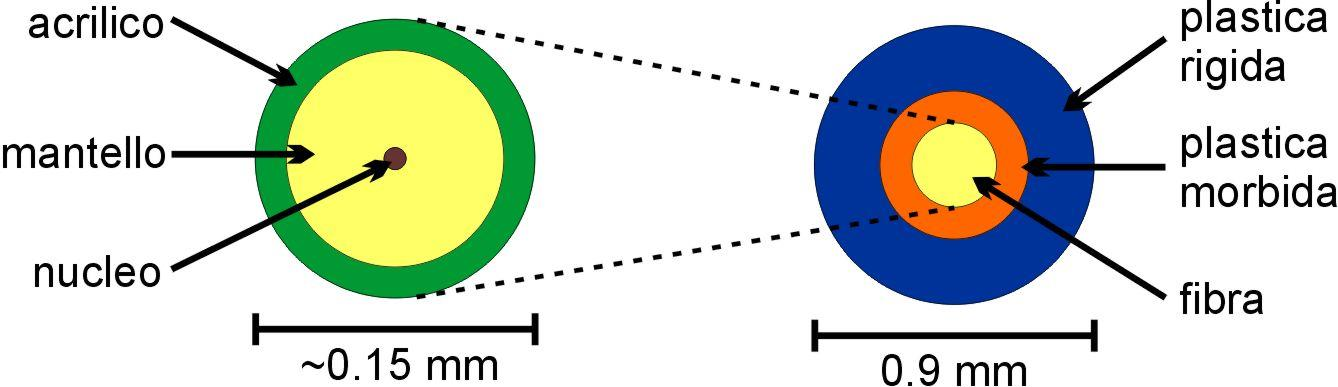
\includegraphics[width=0.6\textwidth]{Images/fig-022.png}
    \caption{Cross-section showing bare fiber (left, $\sim$0.15 mm) and 900-micron buffered fiber (right, 0.9 mm). The buffer provides mechanical protection using soft and rigid plastic layers.}
    \label{fig:buffer_900}
\end{figure}

This cable type is mainly used in devices and compound cables.

\subsubsection{Fiber Ribbons}

Bare fibers can be grouped in \textbf{flat ribbons} containing 2, 4, 8, or 12 fibers. This structure simplifies the management and splicing of multi-fiber cables.

\begin{figure}[H]
    \centering
    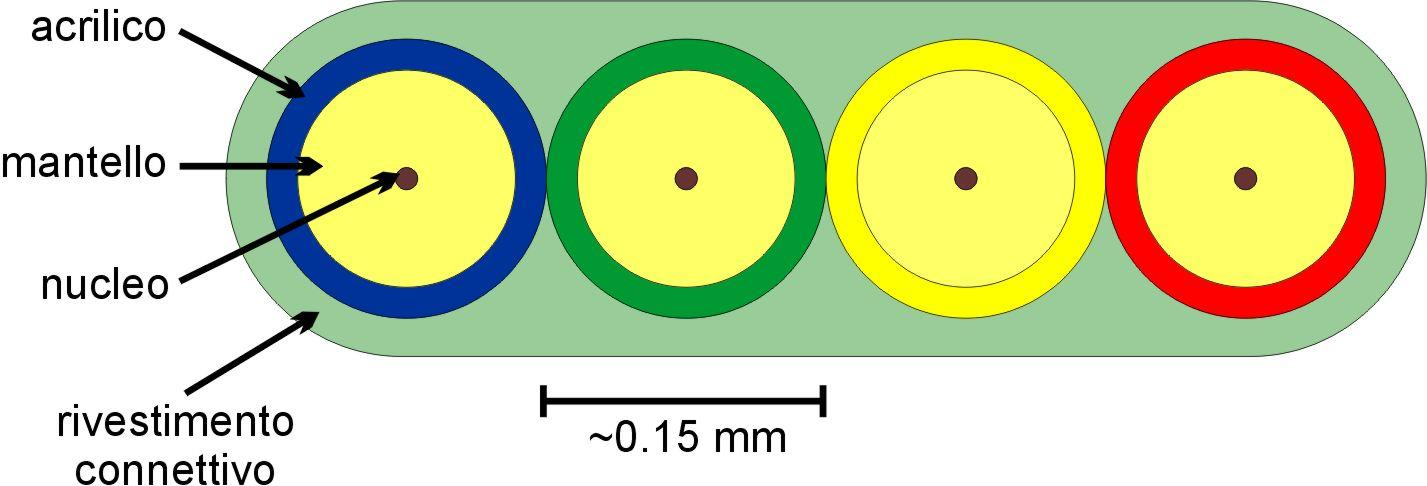
\includegraphics[width=0.7\textwidth]{Images/fig-021.png}
    \caption{Cross-section of a fiber ribbon containing 4 fibers. Each fiber consists of core, cladding, and acrylic coating, all embedded in a connective coating. The ribbon structure simplifies mass fusion splicing.}
    \label{fig:fiber_ribbon}
\end{figure}

\subsection{Patch Cords}

Patch cords installed in ``safe'' locations are usually protected by a sheathing that encloses one or more 900-micron buffered fibers surrounded by \textbf{aramid yarn} (usually Kevlar), which withstands traction forces.

\subsection{Multi-Fiber Cables}

In multi-fiber cables, the fibers are housed either:
\begin{itemize}
    \item In \textbf{tubes} wrapped around a supporting central dielectric rod
    \item In \textbf{slots} carved in the rod itself
\end{itemize}

The central rod also serves the fundamental role of \textbf{contrasting thermal expansion} (or contraction) of the cable.

\begin{figure}[H]
    \centering
    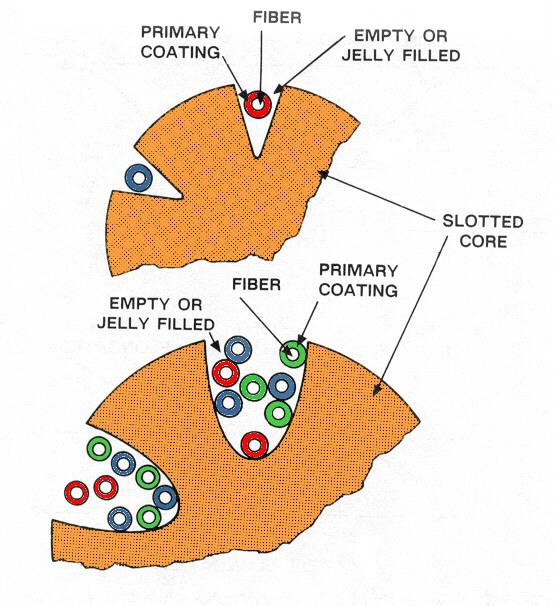
\includegraphics[width=0.7\textwidth]{Images/fig-029.png}
    \caption{Cross-sectional view of multi-fiber cable structures showing fiber placement in tubes or slotted cores. The fibers can be empty or jelly-filled for additional protection.}
    \label{fig:multifiber_structure}
\end{figure}

\subsection{Cable Protection Layers}

Cables have different protecting layers with various functionalities:

\begin{figure}[H]
    \centering
    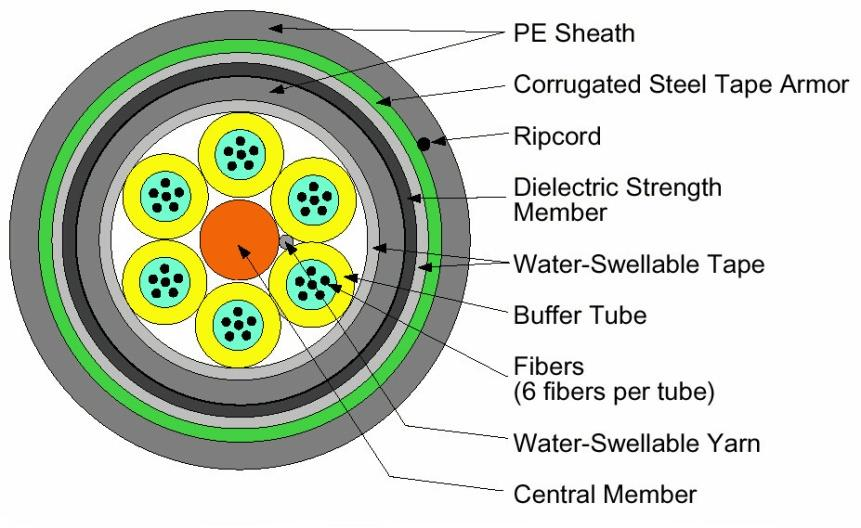
\includegraphics[width=0.75\textwidth]{Images/fig-033.png}
    \caption{Detailed cross-section of a multi-fiber optical cable showing all protection layers: PE sheath, corrugated steel tape armor, ripcord, dielectric strength member, water-swellable tape, buffer tubes with fibers, water-swellable yarn, and central member.}
    \label{fig:cable_layers}
\end{figure}

Key protective elements include:

\begin{itemize}
    \item \textbf{Water-swellable tape:} Expands when in contact with water, preventing water infiltration if the external sheathing is damaged
    \item \textbf{Metallic armoring:} Protects against accidental hits and rodents
    \item \textbf{PE (Polyethylene) sheath:} Outer protective layer
    \item \textbf{Ripcord:} Facilitates cable opening
    \item \textbf{Dielectric strength members:} Provide mechanical strength without conducting electricity
\end{itemize}

\begin{figure}[H]
    \centering
    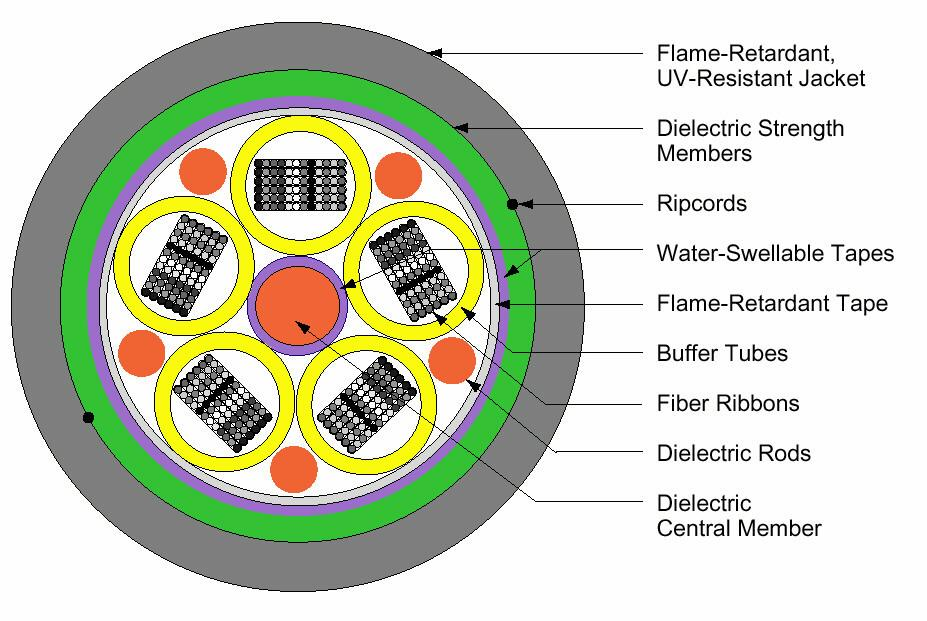
\includegraphics[width=0.75\textwidth]{Images/fig-035.png}
    \caption{Cross-section of a high-capacity ribbon cable showing flame-retardant UV-resistant jacket, dielectric strength members, water-swellable tapes, buffer tubes containing fiber ribbons, and central member.}
    \label{fig:ribbon_cable}
\end{figure}

\subsection{High-Density Cables}

Commercial cables can contain up to 300 or more fibers:

\begin{figure}[H]
    \centering
    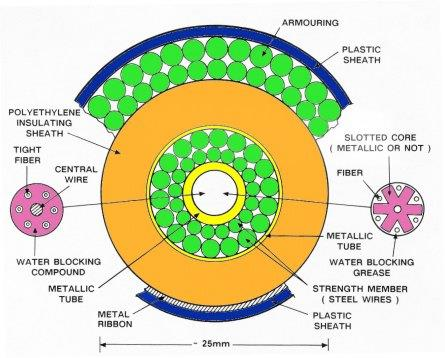
\includegraphics[width=0.55\textwidth]{Images/fig-041.png}
    \caption{Cross-section of a submarine cable with metallic armoring showing the complex structure of protection layers including polyethylene insulating sheath, tight fibers in slotted core, metallic tubes, water blocking compound, and strength members.}
    \label{fig:high_density_cable}
\end{figure}

Example configuration: 300 fibers grouped in 5 tubes, each bearing 5 ribbons with 12 fibers each.

\subsection{Cable Installation Methods}

\subsubsection{Underground Installation}

\begin{figure}[H]
    \centering
    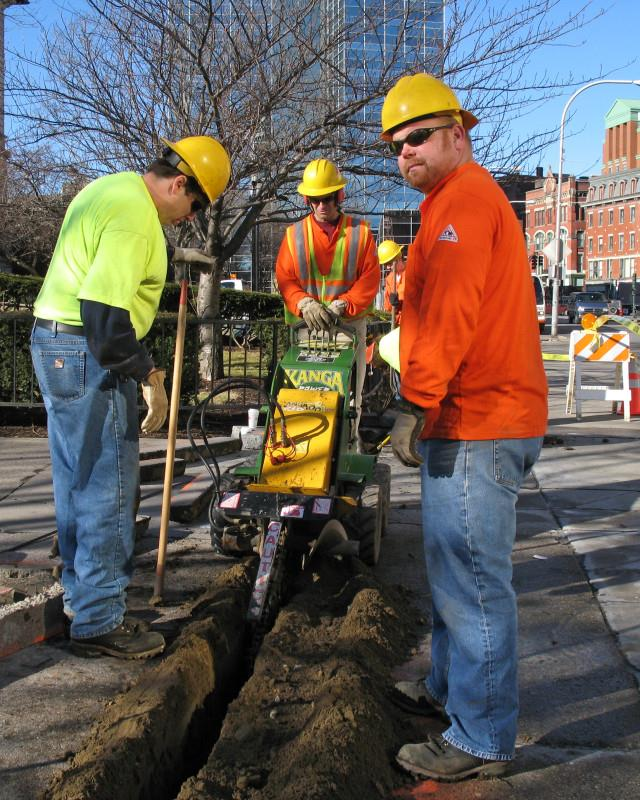
\includegraphics[width=0.55\textwidth]{Images/fig-037.png}
    \caption{Underground cable installation using micro-trenching technique. Workers use specialized equipment to create narrow trenches in urban environments for fiber optic cable placement.}
    \label{fig:microtrenching}
\end{figure}

\subsubsection{Aerial Cables}

Metallic cables housing optical fibers can be installed in lieu of shield (or earth) wire along high-voltage electric lines. Aerial installations can also use self-bearing cables with a standardized \textbf{Figure-8} shape.

\begin{figure}[H]
    \centering
    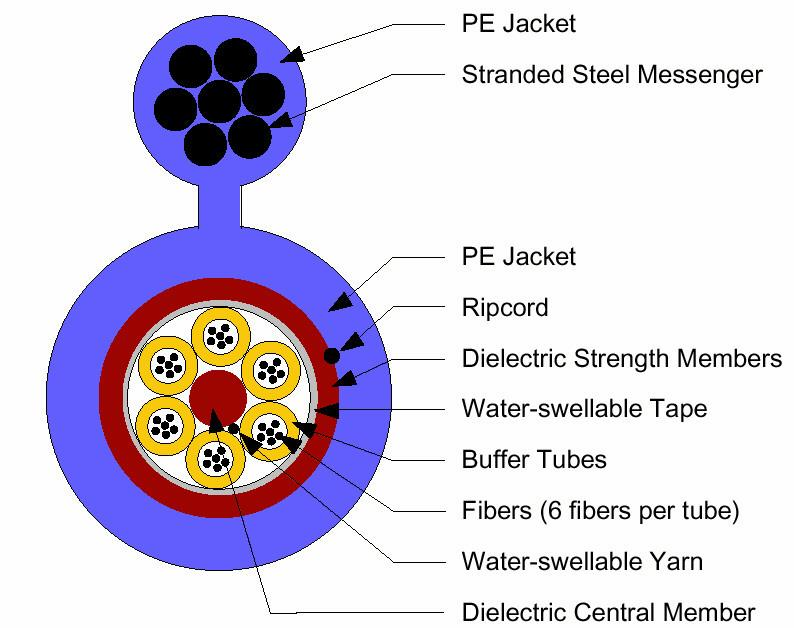
\includegraphics[width=0.6\textwidth]{Images/fig-040.png}
    \caption{Cross-section of a Figure-8 aerial cable design showing the stranded steel messenger for mechanical support and the optical cable portion with buffer tubes, dielectric members, and protective layers.}
    \label{fig:figure8_cable}
\end{figure}

\subsubsection{Submarine Cables}

Submarine cables are heavily armored to withstand:
\begin{itemize}
    \item The installation process
    \item High pressure at the sea bed
    \item Accidental impacts from anchors and drag-nets
\end{itemize}

Close to the coast, cable protection is increased by reinforcing the armoring or burying the cable in the sea bed. Submarine cables often include \textbf{electric wires} to remotely power optical fiber amplifiers.

\begin{figure}[H]
    \centering
    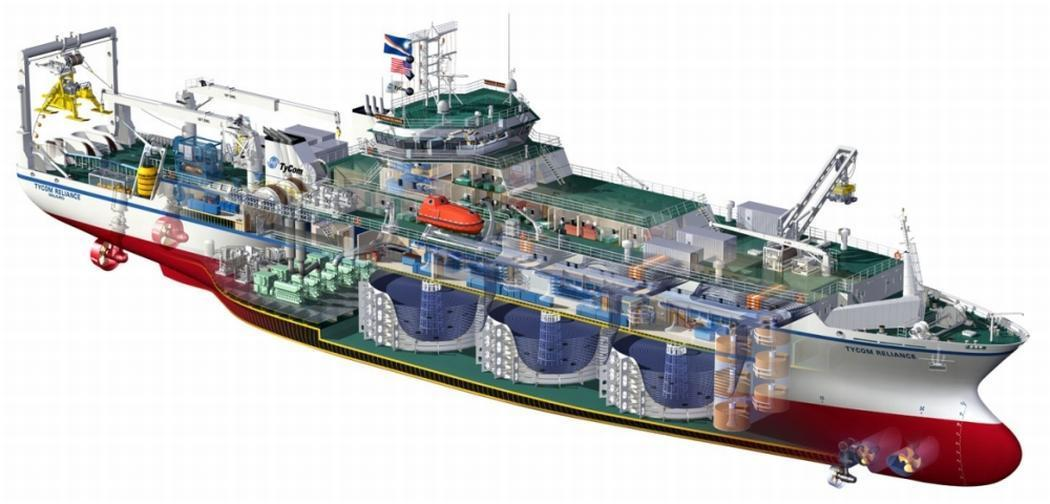
\includegraphics[width=0.85\textwidth]{Images/fig-044.png}
    \caption{Modern cable-laying ship (Giulio Verne, Pirelli Cables and Systems) showing the specialized equipment and cable storage facilities required for submarine cable installation.}
    \label{fig:cable_ship}
\end{figure}

\begin{figure}[H]
    \centering
    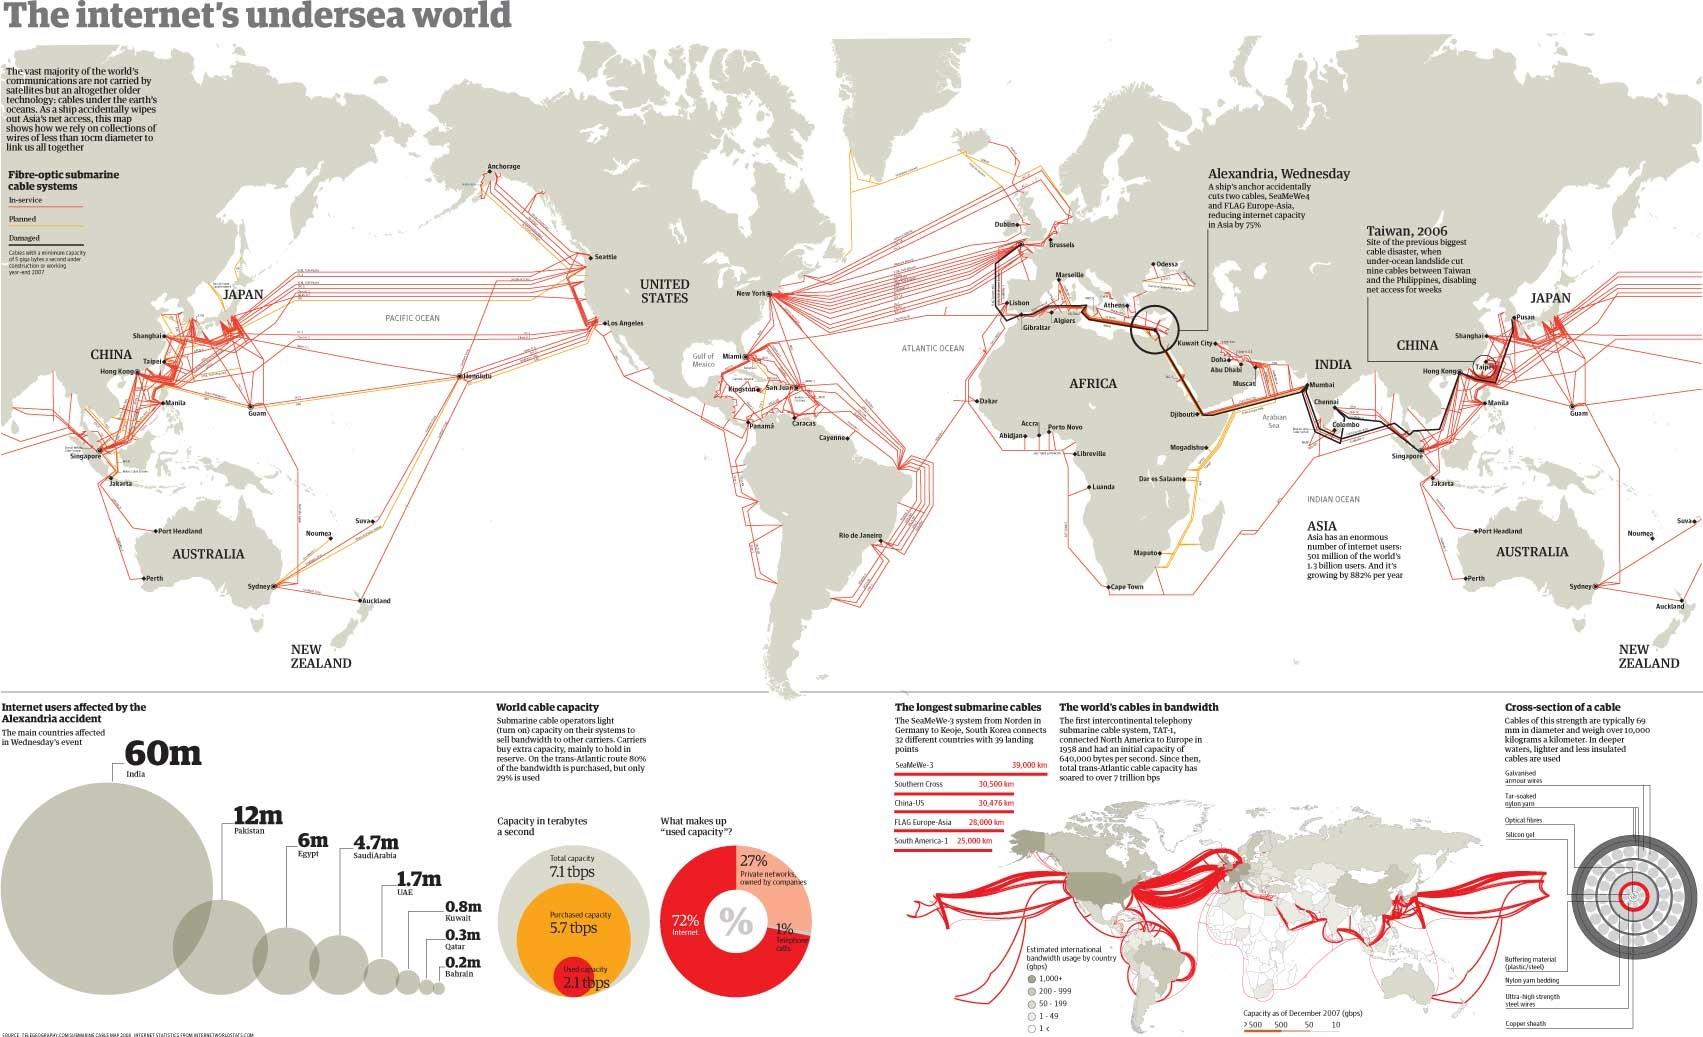
\includegraphics[width=0.9\textwidth]{Images/fig-046.png}
    \caption{Global submarine cable network map showing the extensive undersea fiber optic infrastructure connecting continents. This network forms the backbone of international internet and telecommunications.}
    \label{fig:submarine_network}
\end{figure}

% ==================== CONCLUSIONS ====================
\section{Conclusions}

The production of optical fibers is a sophisticated multi-stage process that requires:

\begin{enumerate}[leftmargin=*]
    \item \textbf{Precise control of chemical reactions} during preform production to achieve ultra-high purity silica with controlled dopant profiles
    
    \item \textbf{Accurate thermal and mechanical control} during fiber drawing to maintain consistent diameter and optical properties
    
    \item \textbf{Appropriate protection strategies} during cabling to ensure fiber survival in various deployment environments
\end{enumerate}

The choice of CVD technique depends on the application requirements:

\begin{itemize}
    \item \textbf{MCVD/PCVD:} Suitable for specialty fibers requiring precise index profiles
    \item \textbf{OVD/VAD:} Preferred for high-volume production of standard telecom fibers
\end{itemize}

Modern production facilities can produce hundreds of kilometers of fiber from a single preform, with drawing speeds reaching tens of meters per second.

\end{document}
